\documentclass[10pt]{article}
\usepackage{a4}
\usepackage{epsfig}
\usepackage{listings}
\lstset{language=Delphi}%
\lstset{basicstyle=\sffamily\small}%
\lstset{commentstyle=\itshape}%
\lstset{keywordstyle=\bfseries}%
%\lstset{blankstring=true}%
\newif\ifpdf
\ifx\pdfoutput\undefined
  \pdffalse
\else
  \pdfoutput=1
  \pdftrue
\fi
\begin{document}
\title{Programming GTK in Free Pascal}
\author{Florian Kl\"ampfl\\and\\Micha\"el Van Canneyt}
\date{September 2000}
\maketitle
\section{Introduction}
In this second article on programming the GTK toolkit, a more advanced use
of the GTK library is presented. Techniques to create a new GTK widget
are discussed by creating two custom widgets. 

The first widget is realized by combining existing GTK widgets to create 
a new widget, a GTKFileEdit component, modeled after the TFileEdit component
found in the RXLib library for Delphi.

When constructing the second widget, the focus will be on how a widget
should draw itself in GTK.

\section{Preliminaries}
Whatever the method used when creating new GTK widgets, it is necessary to 
split the functionality of the widget in 2 parts. 
The first part is the functionality that is common to all instances of the 
new widget. This part is by far the most important one, and is implemented 
in the 'class record'. This record will be initialized with a class 
initialization function. It will also contain pointers to callbacks to
draw a particular instance or callbacks to react on user events.

The second part concerns the particular instance of the widget that is 
created, it contains the data that determines the state of an instance
after it is created, it is the actual object created by the user. This 
part of the widget is implemented in the 'Object record'. For this record
also there is a initialization function.

When the two records have been defined, some standard methods must be 
implemented in order to integrate the new widget in the GTK library. 
Implementing some methods for the user to manipulate the properties 
of the new widget finishes the creation of a new widget.

Since GTK is implemented in C, the programmer must obey some rules in order
to preserve the object-oriented aspect of the GTK library. More precisely,
when defining the class and object records, care must be taken to specify 
the parent object or class as the first element in the newly created structure. This
will allow typecasting of the widget to its parent objects.

Taking a look at the \lstinline|TGtkContainer| widget, we see that the declaration
of the object record starts with the declaration of its parent widget 
\lstinline|TGtkWidget|:
\begin{lstlisting}{}
TGtkContainer = record
  widget : TGtkWidget;
  focus_child : PGtkWidget;
  flag0 : longint;
  resize_widgets : PGSList;
end;
\end{lstlisting}
The same is true for the \lstinline|TGtkContainerClass| record:
\begin{lstlisting}{}
TGtkContainerClass = record
  parent_class : TGtkWidgetClass;  
  n_child_args : guint;
  // ...
end;
\end{lstlisting}
For both the components that will be made, such records will be made.

\section{A filename edit component}
The \lstinline|TGTKFileEdit| component presented here is composed out of three 
other components; first of all a single line edit control, in which the
user can type a filename if he wishes. The second is a button. The button
is always placed on the right edge of the edit control, and has the same
height. The third component is an image component, which is used to display
an image on the button\footnote{In GTK a button does not necessarily contains a
caption, it is an empty placeholder, which can be filled with whatever 
you want, in this case an image. To have the button display a caption, 
a label is placed in it.}

Since the edit and button component must be kept together, we use a
\lstinline|TGtkHBox| as the 'Parent' component, and this component will be
used to keep the edit and button control. There is no need to consider the
image component, since it will be placed inside the button.

Having decided that, the structure of the record for the instance of the
component is more or less determined:
\begin{lstlisting}{}
Type
  PGtkFileEdit = ^TGtkFileEdit;
  TGtkFileEdit = Record
    Box : TGtkHBox;
    Edit : PGtkEntry;
    Button : PGtkButton;
    Image : PGtkPixmap;
    Dialog : PGtkFileSelection;
  end;
\end{lstlisting}
The first field of the record contains the parent record, as required
by the OOP structure of GTK. The other fields are used to contain references
to the other controls used. The \lstinline|Dialog| field will be filled with the
reference to the file selection dialog which is created when the user clicks
the button, at all other times it will contain a \lstinline|nil| pointer.
Remark that the first field is a record, and all other fields are pointers.

Since the fields of the record are 'Public' the user can access the button
and edit components, and set or read their properties, and set additional 
signals. (e.g. a 'change' signal for the edit component)

The class record for the {TGTKFileEdit} component should contain as a first 
field the parent class record, in this case \lstinline|TgtkHBoxClass|. Furthermore
in the class record the default bitmap that will be displayed on the button
will be stored. For this two fields are needed; one to keep the bitmap
(\lstinline|DefaultPixmap|, and
another one to keep a bitmask that is used to determine the transparent
pixels in the bitmap (\lstinline|DefaultBitMap|):
\begin{lstlisting}{}
  PGtkFileEditClass = ^TGtkFileEditClass;
  TGtkFileEditClass = Record
    Parent_Class : TgtkHBoxClass;
    DefaultPixmap : PGdkPixmap;
    DefaultBitMap : PGdkBitmap;
  end;
\end{lstlisting}
As usual, a pointer type is defined which points to the record. The fields
of the class record will be filled in by the initialization code for our
component, as will be shown below.

A new widget must be registered with GTK by calling the
\lstinline|gtk_type_unique| function. This function returns a unique
identifier that can be used to refer to your new widget. This value
must be accessible when creating new instances.

Usually, this is done by registering the component with the GTK library
inside a function which returns this unique ID to the user:
The \lstinline|GtkFileEdit_get_type| function. 
When this function is called for the first time, it will register
the new class with GTK, which will in turn supply a unique ID for the
new component. This ID is returned and also stored, and will be returned
the next times when the \lstinline|GTKFileEdit_get_type| function is called.

The \lstinline|GTKFileEdit_get_type| function looks like this
\lstinline|gtk\_type\_unique|:
\begin{lstlisting}{}
Function GtkFileEdit_get_type : Guint;cdecl;

Const
  GtkFileEditInfo : TGtkTypeInfo =
    (type_name : 'GtkFileEdit';   
     object_size : SizeOf(TGtkFileEdit);
     class_size : SizeOf(TGtkFileEditClass);
     class_init_func : TGtkClassInitFunc(@GtkFileEditClassInit);
     object_init_func : TGtkObjectInitFunc(@GtkFileEditInit);   
     reserved_1 : Nil;
     reserved_2 : Nil;
     base_class_init_func : Nil
    );

begin
  if (GtkFileEditType=0) then
    GtkFileEditType:=gtk_type_unique(gtk_hbox_get_type,@GtkFileEditInfo);
  Result:=GtkFileEditType;  
end;
\end{lstlisting}
Registering the new widget is done by passing a \lstinline|TGtkTypeInfo| 
record to \lstinline|gtk_type_unique|, where the fields of this record 
are filled with the following information:
\begin{description}
\item[type\_name] Contains the name of the type that must be registered. 
\item[object\_size] The size of the object record. GTK itself will allocate 
the memory when an new instance of the object is created, so it must know the
size of the object.  
\item[class\_size] The size of the class object. Only one instance of this
record will be created (by GTK)
\item[class\_init\_func] The address of a function that will initialize the
class record. This function accepts as a single argument a pointer to the
class record to be initialized. This function will normally be called only
once.
\item[object\_init\_func] The address of a function that will initialize 
an instance of the object. The function must accept as a single argument
a pointer to an instance of the object. This instance will be created by 
GTK. This function is called for each instance of the object.
\end{description}
The other three fields of the record are unfortunately not documented, so
they are left blank. 

Along with the \lstinline|TGtkTypeInfo| record, the tyoe the type of the 
parent class (acquired with its own \lstinline|gtk_hbox_get_type| 
function) is passed to the \lstinline|gtk_type_unique| function. 

If a \lstinline|class_init_func| was specified when registering the new type,
then GTK will call this method; it should initialize any class-specific 
data in the class record. In the case of the \lstinline|GTKFileEdit|, the bitmap 
which is used to fill the button is loaded:
\begin{lstlisting}{}
Procedure GtkFileEditClassInit (CObj : PGtkFileEditClass);cdecl;
   
begin
  With Cobj^ do
    DefaultPixMap:=gdk_pixmap_create_from_xpm(Nil,@DefaultBitmap,
                                              Nil,'fileopen.xpm');
end;
\end{lstlisting}
The \lstinline|gdk_pixmap_create_from_xpm| does 2 things: It loads a bitmap
from the \textsf{fileopen.xpm} file and returns a PGdkPixmap pointer.
At the same time it returns a pointer to a bitmask which designates the
transparent regions of the bitmap.

The result of this function is stored in the class record, so the bitmap
is available when a new instance of the class is created.

The \lstinline|GtkFileEditClassInit| and \lstinline|GtkFileEdit_get_type| 
functions are not called automatically by GTK. There are basically
2 solutions to do this as described below.

The first one is specific to Free Pascal: the \lstinline|GtkFileEdit_get_type|
can be called from the unit initialization code; This means that the objects 
are registered with GTK, even if they're not used. It also means that the
GTK library must be initialized first, and hence should also be initialized
in the initialization code of some unit.

The second method is the method used in C: The function to create a new
instance of the \lstinline|TGTKFileEdit| class, \lstinline|GTKFileEdit_new|,
calls the \lstinline|get_type| function to register the class if needed,
as follows:
\begin{lstlisting}{}
Function GtkFileEdit_new : PGtkWidget;cdecl;

begin
  Result:=gtk_type_new(GtkFIleEdit_get_type)
end;
\end{lstlisting}
When the first instance of the \lstinline|GTKFileEdit| widget is created, the 
call to \lstinline|GtkFileEdit_get_type| will register the widget class 
first. Subsequent calls to create a new instance will just use the stored 
value of the ID that identifies the \lstinline|GTKFileEdit| class.

To be able to create an instance of the \lstinline|GTKFileEdit| class, one
more procedure must be implemented, as can be seen from the class
registration code: \lstinline|GtkFileEditInit|. This procedure will 
initialize (i.e. create) a new instance of the class; it should do
whatever is necessary so the instance is ready for use.

In the case of the \lstinline|GTKFileEdit| class, this simply means that
all widgets of which the class is composed, must be created and placed to
gether. This is shown in the following code:
\begin{lstlisting}{}
Procedure GtkFileEditInit (Obj : PGtkFileEdit);cdecl;

Var
  PClass : PGtkFileEditClass;

begin
  PClass:=PGtkFileEditClass(PGtkObject(Obj)^.klass);
  With Obj^ do
    begin
    Edit := PgtkEntry(gtk_entry_new);
    Button := PgtkButton(gtk_button_new);
    Image := PgtkPixMap(gtk_pixmap_new(PClass^.DefaultPixmap,
                                       PClass^.DefaultBitmap));
    gtk_container_add(PGtkContainer(Button),PGtkWidget(Image));
    gtk_box_pack_start(PgtkBox(Obj),PGtkWidget(Edit),True,True,0);
    gtk_box_pack_start(PgtkBox(Obj),PGtkWidget(Button),False,True,0);
    gtk_signal_connect(PgtkObject(Button),'clicked',
                       TGtkSignalFunc(@GtkFileEditButtonClick),Obj);
    end;
  gtk_widget_show_all(PGtkWidget(Obj));
end;
\end{lstlisting}
The code is self explanatory; the sub-widgets are created, and a reference
to them is stored in the fields of our instance record. Note that the
ancestor (a \lstinline|gtkHbox|) is not initialized, this has been done 
already by the OOP mechanism of GTK. 

After the objects are created, they are put together in the horizontal 
box, with the options chosen in such a way that the composed widget scales
well if needed. The bitmap image is of course placed in the button.

Lastly, a signal handler is added to the button, so that when it is clicked,
we can take appropriate action (i.e. show a dialog to select a file). 
Note that as the \lstinline|Data| parameter for the signal, the reference 
to the \lstinline|GTKFileEdit| instance is passed.

Now the class is ready to be created and shown. However, it doesn't do
anything useful yet. The callback for the button click must still be used.

The callback for the button must create a file selection dialog, show it,
and when it has been closed by a click on the 'OK' button, it should set
the text of the edit widget to the name of the selected file.

In order to do this, some extra callbacks are needed, as can be seen in the
following code:
\begin{lstlisting}{}
Procedure GtkFileEditButtonClick (Obj : PGtkObject; Data : PgtkFileEdit);cdecl;

Var
  Dialog : PGtkFileSelection;
  
begin
  Dialog := PGtkFileSelection(gtk_file_selection_new('Please select a file'));
  Data^.Dialog:=Dialog;
  gtk_signal_connect(PGTKObject(Dialog^.ok_button),'clicked',
                     TGTKSignalFunc(@GtkStoreFileName),data);
  gtk_signal_connect_object (PGtkObject((Dialog)^.ok_button),'clicked', 
                            TGTKSIGNALFUNC (@gtk_widget_destroy), PgtkObject(Dialog));
  gtk_signal_connect_object (PGtkObject((Dialog)^.cancel_button),'clicked', 
                            TGTKSIGNALFUNC (@gtk_widget_destroy), PgtkObject(Dialog));
  gtk_widget_show(PgtkWidget(dialog));
end;
\end{lstlisting}
The listing shows that an instance of the file selection dialog is created,
and that its signals are set up so that when the user clicks the 'Cancel'
button, the file selection dialog is simply destroyed, and when the 'OK'
button is selected, first a callback is called in which the name of the
selected file will be retrieved, and secondly the file selection dialog
is destroyed. 
Two remarks concerning this code are in order:
\begin{enumerate}
\item The order in which the signals are connected to the 'clicked' event of 
the OK button is important, since they will be triggered in the order that
they were connected.
\item A reference to the dialog is stored in the \lstinline|GTKFileEdit|
instance, and the reference to the \lstinline|GTKFileEdit| is passed as the
\lstinline|Data| parameter of the signal. 
\end{enumerate}
Finally, when the 'OK' button of the file selection dialog is clicked, the
following callback is executed to store the filename in the edit widget of
the \lstinline|GTKFileEdit| widget:
\begin{lstlisting}{}
Procedure GtkStoreFileName(Button : PgtkButton; 
                           TheRec : PGtkFileEdit); cdecl;

begin
  With TheRec^ do 
    begin
    gtk_entry_set_text(Edit,gtk_file_selection_get_filename(Dialog));
    Dialog:=Nil;
    end;
end;
\end{lstlisting}
The callback also removes the reference to the file selection dialog. This
could also have been done by explicitly setting a 'destroy' signal handler
for the dialog, but since the dialog is destroyed after the 'OK' button is 
clicked, it is done here.

Now the \lstinline|GTKFileEdit| is ready for use. It is possible to add 
some utility functions to the class, for instance one to get or set set 
the filename:
\begin{lstlisting}{}
Procedure GtkFileEdit_set_filename (Obj : PGtkFileEdit; FileName : String);cdecl;

begin
  gtk_entry_set_text(Obj^.Edit,PChar(FileName));
end;

Function GtkFileEdit_get_filename (Obj : PGtkFileEdit) : String;cdecl;

begin
  Result:=StrPas(gtk_entry_get_text(Obj^.Edit));
end;  
\end{lstlisting}
The widget can now be used like any other GTK widget:
\begin{lstlisting}{}
program ex1;

{$mode objfpc}

uses
 glib,gtk,fileedit;

procedure destroy(widget : pGtkWidget ; data: pgpointer ); cdecl;
begin
  gtk_main_quit();
end;

var
  window,
  fileed,
  box,
  Button : PgtkWidget;
      
begin
  gtk_init (@argc, @argv);
  window := gtk_window_new (GTK_WINDOW_TOPLEVEL);
  fileed := gtkfileedit_new;
  gtk_container_set_border_width(GTK_CONTAINER(Window),5);
  box:=gtk_vbox_new(true,10);
  button:=gtk_button_new_with_label('Quit');
  gtk_box_pack_start(pgtkbox(box),PGtkWidget(fileed),False,False,0);
  gtk_box_pack_start(pgtkbox(box),pgtkWidget(button),True,False,0);
  gtk_container_add(GTK_Container(window),box);
  gtk_signal_connect (PGTKOBJECT (window), 'destroy',
                      GTK_SIGNAL_FUNC (@destroy), NULL);
  gtk_signal_connect_object(PgtkObject(button),'clicked',
                      GTK_SIGNAL_FUNC(@gtk_widget_destroy),
                      PGTKOBJECT(window));
  gtk_widget_show_all (window);
  gtk_main ();
end.
\end{lstlisting}
The result will look something like figure \ref{fig:fileedit}

\begin{figure}[h]
\begin{center}
\caption{The GTKFileEdit in action}\label{fig:fileedit}
\vspace{3mm}
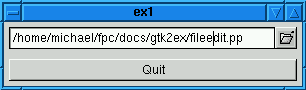
\epsfig{file=gtk2ex/ex1.png}
\end{center}
\end{figure}    

This widget is of course not finished, it can be enhanced in many ways:
Some additional functionality would be to provide a filter for the dialog,
or to set the directory initialiy displayed, provide a title for the dialog,
set a different image on the button, verify that the selected file exists, 
and so on. these can be added in much the same way that the
\lstinline|GTKFileEdit_get_filename| and
\lstinline|GTKFileEdit_set_filename| were implemented.

The fact that the parts making up the widget, such as the button and the edit
widgets, are available as fields in the instance record makes it possible
for the user to set additional properties, provided by these widgets. One
could imagine the user connecting to the 'changed' signal of the edit, to
check whether or not the filename being typed exists, and enabling or 
disabling other widgets accordingly. The usage of the file selection dialog
itself also makes this clear. 

\section{A LED digit widget}
The second widget to be presented in this article is a widget displaying 
a LED digit; such as found in many CD-Player displays or digital clocks.
This will demonstrate how to draw a widget on the screen.

A descendent which reacts to mouse clicks will also be created, which will
demonstrate how to react to user events such as mouse clicks.

A digit consists out of 7 segments, which can be either lit or not lit
(dimmed). For each of the 10 digits (0..9) the state of each of the segments
must be specified. For this we introduce some types and constants:
\begin{lstlisting}{}
Type
  TLEDSegment = (lsTop,lsCenter,lsBottom,
                 lsLeftTop,lsRightTop,
                 lsLeftBottom, lsRightBottom);
  TLedSegments = Array[TLedSegment] of boolean;
  
Const 
  DigitSegments : Array[0..9] of TLEDSegments = 
    (
     (true,false,true,true,true,true,true),       // 0
     (false,false,false,false,true,false,true),   // 1
     (true,true,true,false,true,true,false),      // 2                
     (true,true,true,false,true,false,true),      // 3
     (false,true,false,true,true,false,true),     // 4
     (true,true,true,true,false,false,true),      // 5
     (true,true,true,true,false,true,true),       // 6
     (true,false,false,false,true,false,true),    // 7
     (true,true,true,true,true,true,true),        // 8
     (true,true,true,true,true,false,true)        // 9
    );
\end{lstlisting}
The meaning of each of these types and the constant is obvious.

Each segment is drawn between 2 points, located on a rectangle
with 6 points, as shown in figure \ref{fig:corners}
\begin{figure}
\begin{center}
\caption{Corners of a digit}\label{fig:corners}
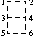
\epsfig{file=gtk2ex/corners.png}
\end{center}
\end{figure}
Each segment is drawn between 2 corners: a start corner and an end corner.
For each segment the start and end corner are stored in the 
\lstinline|SegmentCorners| array.
\begin{lstlisting}{}
Type
  TSegmentCorners = Array [1..2] of Byte;

Const
  SegmentCorners : Array [TLEDSegment] of TSegmentCorners = 
    (
     (1,2),
     (3,4),
     (5,6),
     (1,3),
     (2,4),
     (3,5),
     (4,6)
    );
\end{lstlisting}
These constants will facilitate the drawing of the digit later on. 

For the digit widget, 2 records must again be introduced; one for the class,
and one for the instances of objects:
\begin{lstlisting}{}
Type
  TPoint = Record 
    X,Y : gint;
    end;

  PGtkDigit = ^TGtkDigit;  
  TGtkDigit = Record 
    ParentWidget : TGtkWidget;
    borderwidth,
    digit : guint;
    Corners : Array [1..6] of TPoint;
  end;
  
  PGtkDigitClass = ^TGtkDigitClass;
  TGtkDigitClass = Record
    Parent_Class : TGtkWidgetClass;
  end;
\end{lstlisting}
The class record \lstinline|TGtkDigitClass| contains no extra information
in this case, it has the parent class record as its ony field, as required 
bythe GTK object model. It could however be used to store some default values to 
be applied to new widgets, as was the case for the \lstinline|GTKFileEdit|
widget.

The object record contains three extra fields:
\begin{description}
\item[borderwidth] The distance between the segments and the border of 
the widget.
\item[digit] The digit to be displayed.
\item[Corners] this array contains the locations of each of the corners
between which the segments will be drawn.
\end{description}
The \lstinline|GTKDigit| class must be registered with GTK, and this happens
in the same manner as before:
\begin{lstlisting}{}
Function GtkDigit_get_type : Guint;cdecl;

Const 
  GtkDigitInfo : TGtkTypeInfo = 
    (type_name : 'GtkDigit';
     object_size : SizeOf(TGtkDigit);
     class_size : SizeOf(TGtkDigitClass);
     class_init_func : TGtkClassInitFunc(@GtkDigitClassInit);
     object_init_func : TGtkObjectInitFunc(@GtkDigitInit);
     reserved_1 : Nil;
     reserved_2 : Nil;
     base_class_init_func : Nil
    );

begin
  if (GtkDigitType=0) then
    GtkDigitType:=gtk_type_unique(gtk_widget_get_type,@GtkDigitInfo);
  Result:=GtkDigitType;  
end;
\end{lstlisting}
In the class initialization code, the real difference between this widget
and the previous one becomes clear:
\begin{lstlisting}{}
Procedure GtkDigitClassInit (CObj : PGtkDigitClass);cdecl;

begin
  With PGtkWidgetClass(Cobj)^ do 
    begin
    size_request:=@GTKDigitSizeRequest;
    expose_event:=@GTKDigitExpose;
    size_allocate:=@GTKDigitSizeAllocate;
    end;
end;
\end{lstlisting}
Here GTK is told that, in order to determine the size of the widget,
it should first call \lstinline|GTKDigitSizeRequest|; this will provide
GTK with an initial size for the object. After GTK has placed all widgets
in the window, and has determined the sizes and positions it will allocate 
to each widget in the form, it will call \lstinline|GTKDigitSizeAllocate| 
to notify the \lstinline|GTKDigit| widget of the size it is being allocated.

Finally, the \lstinline|expose_event| callback is set; this informs GTK that
when a part of the widget should be drawn (because it is visible to the
user), \lstinline|GTKDigitExpose| should be called. There are actually 2 
callbacks to draw a widget; one of them is
the \lstinline|draw| function and the other is the (here used) 
\lstinline|expose| function. The \lstinline|draw| function of 
\lstinline|GTKWidget| just generates an expose event for the entire widget,
and for the current widget this is enough. There are, however, cases where
it may be necessary to differentiate between the two for optmization
purposes.

The object initialization function \lstinline|| simply initializes all fields to their
default values:
\begin{lstlisting}{}
Procedure GtkDigitInit (Obj : PGtkDigit);cdecl;

Var I : longint;

begin
  gtk_widget_set_flags(pgtkWidget(obj),GTK_NO_WINDOW);
  With Obj^ do
    begin 
    Digit:=0;
    BorderWidth:=2;
    For I:=1 to 6 do
    with Corners[i] do
      begin
      X:=0;
      Y:=0;
      end;
    end;  
end;
\end{lstlisting}
The interesting thing in the initialization function is the call to
\lstinline|gtk_widget_set_flags|; this tells GTK that the
\lstinline|GtkDigit| does not need its own window. Indeed, it will
use its parent window to draw itself when needed.
This also means that no extra resources must be allocated for the widget.

The \lstinline|size_request| callback will in our case simply ask for some
default size for the digit:
\begin{lstlisting}{}
Procedure GTKDigitSizeRequest (Widget : PGtkWidget; 
                               Request : PGtkRequisition);cdecl;
   
Var BW : guint;   
                               
begin
  With PGTKDigit(Widget)^ do
    BW:=BorderWidth;
  With Request^ do
    begin
    Width:=20+2*BW;
    Height:=40+2*BW;
    end;
end;
\end{lstlisting}
usually, GTK will allocate a size at least equal to the size requested. It
may however be more than this.

When GTK has decided what the real size of the widget will be, the
\lstinline|GTKDigitSizeAllocate| will be called:
\begin{lstlisting}{}
procedure GTKDigitSizeAllocate(Widget : PGTKWidget;
                               Allocation : PGTKAllocation);cdecl;
  
begin
  Widget^.Allocation:=Allocation^;
  SetDigitCorners(PGtkDigit(Widget),False);
end;
\end{lstlisting}
This procedure first of all stores the allocated size in the widget, and
then it calls \lstinline|SetDigitCorners| to calculate the positions of
the corners of the segments; this is done as follows:
\begin{lstlisting}{}
Procedure SetDigitCorners(Digit : PGtkDigit; IgnoreOffset : Boolean);

Var
  BW : guint;
  W,H,SX,SY : gint;
  i : longint;
  Widget : PGTKWidget;
  
begin
  Widget:=PGTKWidget(Digit);
  BW:=Digit^.Borderwidth;
  If IgnoreOffset then
    begin
    SX:=0;
    SY:=0;
    end
  else
    begin
    SX:=Widget^.Allocation.x;
    SY:=Widget^.Allocation.y;
    end;
  W:=Widget^.Allocation.Width-2*BW;
  H:=(Widget^.Allocation.Height-2*BW) div 2;  
  With PGTKDigit(Widget)^ do
    For I:=1 to 6 do
      begin
      Case I of
        1,3,5 : Corners[i].X:=SX+BW;
        2,4,6 : Corners[i].X:=SX+BW+W;
      end;
      Case I of
        1,2 : Corners[i].Y:=SY+BW;
        3,4 : Corners[i].Y:=SY+BW+H;
        5,6 : Corners[i].Y:=SY+BW+2*H
      end;
      end;
end;
\end{lstlisting} 
Since the \lstinline|GTKDigit| will draw on its parents window, it must
take into account the offset (x,y) of the allocated size. The reason that
this is parametrized with the \lstinline|IgnoreOffset| parameter will become
clear when the descendent widget is introduced.

This function could be adapted to give e.g. a slight tilt to the digits. 

Remains to implement the \lstinline|expose_event| callback:
\begin{lstlisting}{}
Function GTKDigitExpose (Widget : PGTKWidget;
                         ExposeEvent : PGDKEventExpose) : gint;cdecl;

Var
  Segment : TLedSegment;
     
begin
  With PGTKDigit(Widget)^ do
    For Segment:=lsTop to lsRightBottom do 
      if DigitSegments[Digit][Segment] then
        gdk_draw_line(widget^.window,
                  PgtkStyle(widget^.thestyle)^.fg_gc[widget^.state],
                  Corners[SegmentCorners[Segment][1]].X,
                  Corners[SegmentCorners[Segment][1]].Y,
                  Corners[SegmentCorners[Segment][2]].X,
                  Corners[SegmentCorners[Segment][2]].Y
                  )
      else
        gdk_draw_line(widget^.window,
                  PgtkStyle(widget^.thestyle)^.bg_gc[widget^.state],
                  Corners[SegmentCorners[Segment][1]].X,
                  Corners[SegmentCorners[Segment][1]].Y,
                  Corners[SegmentCorners[Segment][2]].X,
                  Corners[SegmentCorners[Segment][2]].Y
                  );
  
end;
\end{lstlisting}
Here the need for the types and constants, introduced in the
beginning of this section becomes obvious; without them, a huge
case statement would be needed to draw all needed segments. 

Note that when a segment of our digit is not 'lit', it is drawn in the
background color. When the digit to be displayed changes, the segments 
that are no longer lit, must be 'dimmed' again.

Finally we provide 2 methods to get and set the digit to be dislayed:
\begin{lstlisting}{}
Procedure GtkDigit_set_digit (Obj : PGtkDigit; Digit : guint);cdecl;

begin
  if Digit in [0..9] then
    begin
    Obj^.Digit:=Digit;
    gtk_widget_draw(PGTKWidget(Obj),Nil);
    end;
end;

Function GtkDigit_get_digit (Obj : PGtkDigit) : guint;cdecl;

begin
  Result:=Obj^.Digit;
end;  
\end{lstlisting}
Obviously, when setting the digit to be displayed, the widget must be
redrawn, or the display would not change till the next expose event. 
Calling \lstinline|gtk_widget_draw| ensures that the digit will be displayed
correctly. 

Now the widget is ready for use; it can be created and put on a window
in the same manner as the \lstinline|GTKFileEdit| control; the code will
not be shown, but is available separately. 

The result is shown in figure \ref{fig:ex2}.
\begin{figure}
\begin{center}
\caption{The GTKDigit widget in action.}\label{fig:ex2}

\epsfig{file=gtk2ex/ex2.png}
\end{center}
\end{figure}

The widget can be improved in many ways. The segments can be tilted, a
bigger width can be used; the can have rounded edges and so on.

The widget as presented here doesn't react on user events; it has no way
of doing that, since it doesn't have an own window; Therefore a descendent
is made which creates its own window, and which will react on mouse clicks;
this widget will be called \lstinline|GTKActiveDigit|.

The lstinline|GTKActiveDigit| widget is a descendent from its inactive
counterpart. Therefore the class and object records will be (almost) empty:
\begin{lstlisting}{}
Type
  PGtkActiveDigit = ^TGtkActiveDigit;  
  TGtkActiveDigit = Record 
    ParentWidget : TGtkDigit;
    Button : guint8;
  end;
  
  PGtkActiveDigitClass = ^TGtkActiveDigitClass;
  TGtkActiveDigitClass = Record
    Parent_Class : TGtkDigitClass;
  end;
\end{lstlisting}
The \lstinline|Button| field is used to store which button was used to click
on the digit. 

The registration of the new widget is similar to the one for
\lstinline|GTKDigit|, and doesn't need more explanation:
\begin{lstlisting}{}
Const
  GtkActiveDigitType : guint = 0;

Function  GtkActiveDigit_get_type : Guint;cdecl;

Const 
  GtkActiveDigitInfo : TGtkTypeInfo = 
    (type_name : 'GtkActiveDigit';
     object_size : SizeOf(TGtkActiveDigit);
     class_size : SizeOf(TGtkActiveDigitClass);
     class_init_func : TGtkClassInitFunc(@GtkActiveDigitClassInit);
     object_init_func : TGtkObjectInitFunc(@GtkActiveDigitInit);
     reserved_1 : Nil;
     reserved_2 : Nil;
     base_class_init_func : Nil
    );

begin
  if (GtkActiveDigitType=0) then
    GtkActiveDigitType:=gtk_type_unique(gtkdigit_get_type,@GtkActiveDigitInfo);
  Result:=GtkActiveDigitType;  
end;


Function  GtkActiveDigit_new : PGtkWidget;cdecl;

begin
  Result:=gtk_type_new(GtkActiveDigit_get_type)  
end;
\end{lstlisting}
The first real difference is in the class initialization routine:
\begin{lstlisting}{}
Procedure GtkActiveDigitClassInit (CObj : PGtkActiveDigitClass);cdecl;

begin
  With PGtkWidgetClass(Cobj)^ do 
    begin
    realize := @GtkActiveDigitRealize;
    size_allocate := @GtkActiveDigitSizeAllocate;
    button_press_event:=@GtkActiveDigitButtonPress;
    button_release_event:=@GtkActiveDigitButtonRelease;
    end;
end;
\end{lstlisting}
The \lstinline|realize| and \lstinline|size_allocate| of the parent widget
\lstinline|GTKDigit| are overriden here. Also 2 events callbacks are
assigned in order to react on mouse clicks.

The object initialization function must undo some work that was done
ba the parent's initialization function:
\begin{lstlisting}{}
Procedure GtkActiveDigitInit (Obj : PGtkActiveDigit);cdecl;

begin
  gtk_widget_unset_flags(pgtkWidget(obj),GTK_NO_WINDOW);
  With Obj^ do
    Button:=0;
end;
\end{lstlisting}
This is necessary, because the \lstinline|GTKActiveDigit| will create it's
own window.

For this widget, the \lstinline|realize| callback must do a little more
work. It must create a window on which the digit will be drawn. The window
is created with some default settings, and the event mask for the window
is set such that the window will respond to mouse clicks:
\begin{lstlisting}{}
Procedure GtkActiveDigitRealize(widget : PgtkWidget);cdecl;

Var
 attr : TGDKWindowAttr;
 Mask : gint;
 
begin
  GTK_WIDGET_SET_FLAGS(widget,GTK_REALIZED);
  With Attr do
    begin
    x := widget^.allocation.x;
    y := widget^.allocation.y;
    width:=widget^.allocation.width;
    height:=widget^.allocation.height;
    wclass:=GDK_INPUT_OUTPUT;
    window_type:=gdk_window_child;
    event_mask:=gtk_widget_get_events(widget) or GDK_EXPOSURE_MASK or
                GDK_BUTTON_PRESS_MASK OR GDK_BUTTON_RELEASE_MASK;
    visual:=gtk_widget_get_visual(widget);
    colormap:=gtk_widget_get_colormap(widget);
    end;
  Mask:=GDK_WA_X or GDK_WA_Y or GDK_WA_VISUAL or GDK_WA_COLORMAP;
  widget^.Window:=gdk_window_new(widget^.parent^.window,@attr,mask);
  widget^.thestyle:=gtk_style_attach(widget^.thestyle,widget^.window);
  gdk_window_set_user_data(widget^.window,widget);  
  gtk_style_set_background(widget^.thestyle,widget^.window,GTK_STATE_ACTIVE);
end;
\end{lstlisting}
After the window was created, its userdata is set to the widget. This
ensures that the events which occur in the window are passed on to our 
widget by GTK. Finally the background of the window is set to some
other style than the default style.

The size allocation event should in principle do the same as that for the
\lstinline|GTKDigit| widget, with the exeption that the calculation of the
corners for the segments must now not be done relative to the parent window:
\begin{lstlisting}{}
procedure GTKActiveDigitSizeAllocate(Widget : PGTKWidget;
                               Allocation : PGTKAllocation);cdecl;
begin
  Widget^.allocation:=Allocation^;
  if GTK_WIDGET_REALIZED(widget) then
    gdk_window_move_resize(widget^.window,
                           Allocation^.x,
                           Allocation^.y,
                           Allocation^.width,
                           Allocation^.height);
  SetDigitCorners(PGTKDigit(Widget),True);
end;
\end{lstlisting}
This explains the need for the \lstinline|IgnoreOffset| parameter in the
\lstinline|SetDigitCorners| function.

All that is left is to implement the mouse click events:
\begin{lstlisting}{}
Function GtkActiveDigitButtonPress(Widget: PGtKWidget; 
                                    Event : PGdkEventButton) : gint;cdecl;

begin
  PGTKActiveDigit(Widget)^.Button:=Event^.Button;
end;

Function GtkActiveDigitButtonRelease(Widget: PGtKWidget; 
                                      Event : PGdkEventButton) : gint;cdecl;

Var
  Digit : PGtkDigit;
  D : guint;

begin
  Digit:=PGTKDigit(Widget);
  D:=gtkdigit_get_digit(Digit);
  If PGTKActiveDigit(Digit)^.Button=Event^.Button then
    begin
    If Event^.Button=1 then
      GTKDigit_set_digit(Digit,D+1)
    else if Event^.Button=3 then
      GTKDigit_set_digit(Digit,D-1)
    else
      GTKDigit_set_digit(Digit,0);
    end;  
  PGTKActiveDigit(Digit)^.Button:=0;
end;
\end{lstlisting}
As can be seen, the digit will be incremented when the left mouse button
is clicked. The digit is decremented when the right button is clicked. 
On systems with 3 mouse buttons, a click on the middle mouse button will
reset the digit to 0.

After all this, the widget is ready for use, and should look more or less
like the one in figure \ref{fig:ex3}.

\begin{figure}[h]
\begin{center}
\caption{The GTKActiveDigit in action.}\label{fig:ex3}

\epsfig{file=gtk2ex/ex3.png}
\end{center}
\end{figure}

The widgets presented here are not complete; many improvements can be made,
but their main purpose was to demonstrate that implementing some new widgets
is very easy and can be achieved with little effort; what is more, the OOP
structure of GTK is very suitable for the implementation of small
enhancements to existing components, as was shown with the last widget
presented.
\end{document}
